% Created 2013-04-03 Wed 12:53
\documentclass[11pt]{article}
\usepackage[utf8]{inputenc}
\usepackage[T1]{fontenc}
\usepackage{fixltx2e}
\usepackage{graphicx}
\usepackage{longtable}
\usepackage{float}
\usepackage{wrapfig}
\usepackage{soul}
\usepackage{textcomp}
\usepackage{marvosym}
\usepackage{wasysym}
\usepackage{latexsym}
\usepackage{amssymb}
\usepackage{xcolor}
\usepackage{hyperref}
\usepackage{verbatim}
\tolerance=1000
\providecommand{\alert}[1]{\textbf{#1}}

\title{Appendix}
\setlength{\parindent}{0cm}
\hypersetup{
  pdfkeywords={},
  pdfsubject={},
  pdfcreator={Emacs Org-mode version 7.8.11}}

\begin{document}

\maketitle

\setcounter{tocdepth}{3}
\tableofcontents
\vspace*{1cm}

\newpage

\section{Web service API-specifications}
\subsection{M6, Movie Distribution Web Service API Specs}

The web service uses RESTful concepts to provide a standardized and stateless programming interface, for interacting with the system. \\

\textbf{Standard response} \\
All responses consists of the following data:

\begin{table}[H]
\caption{Response message objects}
\begin{center}
\begin{tabular}{|c|l|}
\hline
 Message                     &  Description                                               \\
\hline
 error\_code   &  0 on success, otherwise a number indicating the relevant error.  \\
                             &  NOT TO BE CONFUSED WITH HTTP-Response-code! This   \\
                             &  is assuming the HTTP-Response-code is 200.                \\
\hline
 error\_message  &  A message in English, describing the eventual error.      \\
\hline
Data & Array of data. Usually contains some data object \\
	& (such as users, media etc ..).
\\
\hline
MetaData & Metadata about the data. \\
	& Examples are \texttt{limit}, \texttt{page offset} etc .. \\
\hline
\end{tabular}
\end{center}
\end{table}



\textbf{Security and encoding} \\
All requests should be made with a valid API-key, and values hashed into a “Checksum”. (TODO: Describe hashing details). Requests should be accompanied by a UTC timestamp and a nonce. All authenticated requests should contain an access token.

So every request should look something like: 

\verb[Resource]?auth=[AUTH-STRING]\&parama=xxx\&paramb=yyy \\

Where [AUTH-STRING] is something similar to:
\{ “api-key” : ”AB14” , ”hmac” : ”XZ45” , ”time” : ”213” , “nonce” : “XC98” ; “token” = “DE95” \} \\

The only optional part of this auth object, is the token, which is only used after the user has successfully logged in. \\

\textbf{Objects} \\
Every area of the application has some certain objects with a well defined structure. These are described initially in the relevant section, and utilized throughout the API. This allows for client to receive and process these objects in a uniform manner.\\

\textbf{Parameters} \\
Are GET or POST arguments, depending on the request-type. The parameters documentation consists of a argument name along with a description of the parameter \\

\textbf{Response} \\
Is an associative JSON object, with fields corresponding to the left side column of the table. The right side of the column describes the data in the field of the returned response.
All responses are wrapped in \texttt{Response<TYPE>} objects. For example when calling the \texttt{GET user} method, it returns \texttt{Response<User>}.

\newpage

\subsection{Users (users, tokens, user data \& user groups)}

The users are at the heart of the system. All actions are performed by users, and their identities are associated with both actions and data entities within the system. Users are very simple, but can be extended to application specific needs. This is done by creating new user data types (unique text indexes, that can be used to store data for each user), and assigning data to the users. Tokens are used for accessing the application as a specific user, and is given upon submission of a valid email and password combination.

\begin{table}[H]
\caption{User objects}
\begin{center}
\begin{tabular}{|l|l|}
\hline
 Field                   &  Description                               \\
\hline
 id                      &  The users id                              \\
 \hline
 email                   &  E-mail of the user. False if currently    \\
                         &  logged in user is not permitted to read.  \\
\hline                         
 user\_data  &  All data that exists for this user as an  \\
                         &  associative structure                     \\
\hline
\end{tabular}
\end{center}
\end{table}

\begin{table}[H]
\caption{Token objects}
\begin{center}
\begin{tabular}{|l|l|}
\hline
 Field    &  Description                                    \\
\hline
 token    &  A token string, to be used in further queries  \\
 issued   &  Date and time for issuance                     \\
 expires  &  Date and time for expiration                   \\
\hline
\end{tabular}
\end{center}
\end{table}
 
\begin{tabbing}
\textbf{Get user} \\
\textcolor{black!60}{\textbf{Url structure:}} \hspace{0.2in} \= /user/\{ID\} \\
\textcolor{black!60}{\textbf{Description:}}  \> Who is the user with the id \{ID\}? \\
\textcolor{black!60}{\textbf{Method:}} \> GET \\
\textcolor{black!60}{\textbf{Parameters:}}  \> \textbf{id} Id of the user \\
\textcolor{black!60}{\textbf{Response:}} \> \textbf{Response<User>} \\
\> Response object containing the user object. \\
\end{tabbing}

\begin{center}\line(1,0){250}\end{center}

\begin{tabbing}
\textbf{Get currently logged in user} \\
\textcolor{black!60}{\textbf{Url structure:}} \hspace{0.2in} \= /user/me \\
\textcolor{black!60}{\textbf{Description:}}  \> Who is the currently logged in user? \\
\textcolor{black!60}{\textbf{Method:}} \> GET \\
\textcolor{black!60}{\textbf{Parameters:}}  \> None \\
\textcolor{black!60}{\textbf{Authorization:}} \> Token \\
\textcolor{black!60}{\textbf{Response:}} \> \textbf{Response<User>} \\
\> Response message containing the user object.
\end{tabbing}

\begin{center}\line(1,0){250}\end{center}

\begin{tabbing}
\textbf{Get all users (with parameters)} \\
\textcolor{black!60}{\textbf{Url structure:}} \hspace{0.2in} \= /user?group\_id=\{group\_id\}\&emailFilter=\{emailFilter\}
\\ \> \&limit=\{limit\}\&page=\{page\}\&order\_by=\{order\_by\} \\ \>
\&order=\{order\} \\
\textcolor{black!60}{\textbf{Description:}}  \> Who are the users that match the given parameters \\
\textcolor{black!60}{\textbf{Method:}} \> GET \\
\textcolor{black!60}{\textbf{Parameters:}} \> \textbf{group\_id} Id of a user group. \\ \> Only show users who are members of this/these group(s) \\
\> \textbf{emailFilter} Filter by email \\
\> \textbf{limit} How many users to return? (default = 10) \\
\> \textbf{page} Should there be an offset? \\
\> Default = 1 means no offset. \\
\> \textbf{order\_by} Order by what column? Default = e-mail. \\
\> \textbf{order} Order which way? Default = ASC. \\
\textcolor{black!60}{\textbf{Authorization:}} \> Token \\
\textcolor{black!60}{\textbf{Response:}} \> \textbf{Response<User>} \\
\> Response object containing an array of user objects along \\ \> with page number and count.
\end{tabbing}

\begin{center}\line(1,0){250}\end{center}

\begin{tabbing}
\textbf{Post user access token} \\
\textcolor{black!60}{\textbf{Url structure:}} \hspace{0.2in} \= /user/token/\{email\}/\{password\} \\
\textcolor{black!60}{\textbf{Description:}}  \> Can i have an access-token with these credentials? \\
\textcolor{black!60}{\textbf{Method:}} \> POST \\
\textcolor{black!60}{\textbf{Parameters:}} \> \textbf{email} The users e-mail \\
\> \textbf{password} An SHA-1 hash of the users password. \\
\textcolor{black!60}{\textbf{Response:}} \> \textbf{Response<Token>} \\
\> Response object containing the token.
\end{tabbing}

\begin{center}\line(1,0){250}\end{center}

\begin{tabbing}
\textbf{Renew user access token} \\
\textcolor{black!60}{\textbf{Url structure:}} \hspace{0.2in} \= /user/token/renew \\
\textcolor{black!60}{\textbf{Description:}}  \> Can I renew this token? \\
\textcolor{black!60}{\textbf{Method:}} \> POST \\
\textcolor{black!60}{\textbf{Parameters:}} \> None \\
\textcolor{black!60}{\textbf{Response:}} \> \textbf{Response<Token>} \\
\> Response object containing the renewed token.
\end{tabbing}

\begin{center}\line(1,0){250}\end{center}

\begin{tabbing}
\textbf{Create new user} \\
\textcolor{black!60}{\textbf{Url structure:}} \hspace{0.2in} \= /user \\
\textcolor{black!60}{\textbf{Description:}}  \> Create a new user with this data \\
\textcolor{black!60}{\textbf{Method:}} \> POST \\
\textcolor{black!60}{\textbf{Content-Type}} \> \textbf{application/json} \\
\> \textbf{User} User object.\\
\textcolor{black!60}{\textbf{Response:}} \> \textbf{Response<User>} \\
\> Response object containing the new user.
\end{tabbing}

\begin{center}\line(1,0){250}\end{center}

\begin{tabbing}
\textbf{Delete user} \\
\textcolor{black!60}{\textbf{Url structure:}} \hspace{0.2in} \= /user/\{ID\} \\
\textcolor{black!60}{\textbf{Description:}}  \> Delete the user with this id \\
\textcolor{black!60}{\textbf{Method:}} \> DELETE \\
\textcolor{black!60}{\textbf{Parameters:}} \> \textbf{ID} Id of the user to delete. \\
\textcolor{black!60}{\textbf{Response:}} \> \textbf{Response<User>} \\
\> Response object containing an empty user.
\end{tabbing}

\begin{center}\line(1,0){250}\end{center}

\begin{tabbing}
\textbf{Update user} \\
\textcolor{black!60}{\textbf{Url structure:}} \hspace{0.2in} \= /user/\{ID\}/\{oldPassword\} \\
\textcolor{black!60}{\textbf{Description:}}  \> Update this user with this data \\
\textcolor{black!60}{\textbf{Method:}} \> PUT \\
\textcolor{black!60}{\textbf{Parameters:}} \> \textbf{ID} ID of the user to update. \\
\> \textbf{old-password} The users current password. \\ \> SHA-1 hashed. \\
\textcolor{black!60}{\textbf{Content-Type:}} \> \textbf{application/json} \\
\> \textbf{User} User object with updated user information. \\
\textcolor{black!60}{\textbf{Response:}} \> \textbf{Response<User>} \\
\> Response object containing the updated user.
\end{tabbing}

\begin{center}\line(1,0){250}\end{center}

\begin{tabbing}
\textbf{Get user data} \\
\textcolor{black!60}{\textbf{Url structure:}} \hspace{0.2in} \= /userData/\{userId\} \\
\textcolor{black!60}{\textbf{Description:}}  \> Get user data for the user with the given user id. \\
\textcolor{black!60}{\textbf{Method:}} \> GET \\
\textcolor{black!60}{\textbf{Parameters:}} \> \textbf{userId} Id of the user. \\
\textcolor{black!60}{\textbf{Response:}} \> \textbf{Response<User\_Data>} \\
\> Response object containing the user data.
\end{tabbing}

\begin{center}\line(1,0){250}\end{center}

\begin{tabbing}
\textbf{Create a new user data} \\
\textcolor{black!60}{\textbf{Url structure:}} \hspace{0.2in} \= /userData \\
\textcolor{black!60}{\textbf{Description:}}  \> Make a new user data. \\
\textcolor{black!60}{\textbf{Method:}} \> POST \\
\textcolor{black!60}{\textbf{Parameters:}} \> None. \\
\textcolor{black!60}{\textbf{Content-Type:}} \> application/json. \\
\> \textbf{User\_Data} User data object. \\
\textcolor{black!60}{\textbf{Response:}} \> \textbf{Response<User\_Data>} \\
\> Response object containing the new user data.
\end{tabbing}

\begin{center}\line(1,0){250}\end{center}

\begin{tabbing}
\textbf{Update user data} \\
\textcolor{black!60}{\textbf{Url structure:}} \hspace{0.2in} \= /userData/\{id\} \\
\textcolor{black!60}{\textbf{Description:}}  \> Updates existing user data. \\
\textcolor{black!60}{\textbf{Method:}} \> PUT \\
\textcolor{black!60}{\textbf{Parameters:}} \> \textbf{id} Id of the user data to update. \\
\textcolor{black!60}{\textbf{Response:}} \> \textbf{Response<User\_Data>} \\
\> Response object containing the updated user data.
\end{tabbing}

\begin{center}\line(1,0){250}\end{center}

\begin{tabbing}
\textbf{Delete user data} \\
\textcolor{black!60}{\textbf{Url structure:}} \hspace{0.2in} \= /userData/\{id\} \\
\textcolor{black!60}{\textbf{Description:}}  \> Delete user data with this id \\
\textcolor{black!60}{\textbf{Method:}} \> DELETE \\
\textcolor{black!60}{\textbf{Parameters:}} \> \textbf{id} Id of the user data to delete. \\
\textcolor{black!60}{\textbf{Response:}} \> \textbf{Response<User\_Data>} \\
\> Response object containing empty user data.
\end{tabbing}

\begin{center}\line(1,0){250}\end{center}

\begin{tabbing}
\textbf{Get user group by id} \\
\textcolor{black!60}{\textbf{Url structure:}} \hspace{0.2in} \= /userGroup/\{id\} \\
\textcolor{black!60}{\textbf{Description:}}  \> Gets a user group based on it's id. \\
\textcolor{black!60}{\textbf{Method:}} \> GET \\
\textcolor{black!60}{\textbf{Parameters:}} \> \textbf{id} Id of the user group to get. \\
\textcolor{black!60}{\textbf{Response:}} \> \textbf{Response<UserGroup>} \\
\> Response object containing the user group.
\end{tabbing}

\begin{center}\line(1,0){250}\end{center}

\begin{tabbing}
\textbf{Create a new user group} \\
\textcolor{black!60}{\textbf{Url structure:}} \hspace{0.2in} \= /userGroup \\
\textcolor{black!60}{\textbf{Description:}}  \> Creates a new user group. \\
\textcolor{black!60}{\textbf{Method:}} \> POST \\
\textcolor{black!60}{\textbf{Parameters:}} \> None. \\
\textcolor{black!60}{\textbf{Content-type:}} \> \textbf{application/json} \\
\> \textbf{UserGroup} UserGroup object \\
\textcolor{black!60}{\textbf{Response:}} \> \textbf{Response<UserGroup>} \\
\> Response object containing the new user group.
\end{tabbing}

\begin{center}\line(1,0){250}\end{center}

\begin{tabbing}
\textbf{Update a user group} \\
\textcolor{black!60}{\textbf{Url structure:}} \hspace{0.2in} \= /userGroup/\{id\} \\
\textcolor{black!60}{\textbf{Description:}}  \> Updates an existing user group based on it's id. \\
\textcolor{black!60}{\textbf{Method:}} \> PUT \\
\textcolor{black!60}{\textbf{Parameters:}} \> \textbf{id} Id of the user group to update. \\
\textcolor{black!60}{\textbf{Response:}} \> \textbf{Response<UserGroup>} \\
\> Response object containing the updated user group.
\end{tabbing}

\begin{center}\line(1,0){250}\end{center}

\begin{tabbing}
\textbf{Delete a user group} \\
\textcolor{black!60}{\textbf{Url structure:}} \hspace{0.2in} \= /userGroup/\{id\} \\
\textcolor{black!60}{\textbf{Description:}}  \> Deletes a user group based on it's id. \\
\textcolor{black!60}{\textbf{Method:}} \> DELETE \\
\textcolor{black!60}{\textbf{Parameters:}} \> \textbf{id} Id of the user group to delete. \\
\textcolor{black!60}{\textbf{Response:}} \> \textbf{Response<UserGroup>} \\
\> Response object containing an empty user group object.
\end{tabbing}

\begin{center}\line(1,0){250}\end{center}

\begin{tabbing}
\textbf{Get user's groups} \\
\textcolor{black!60}{\textbf{Url structure:}} \hspace{0.2in} \= /groupOfUser/\{userId\} \\
\textcolor{black!60}{\textbf{Description:}}  \> Gets all groups that a user is member of. \\
\textcolor{black!60}{\textbf{Method:}} \> GET \\
\textcolor{black!60}{\textbf{Parameters:}} \> \textbf{userId} Id of the user. \\
\textcolor{black!60}{\textbf{Response:}} \> \textbf{Response<UserGroup>} \\
\> Response object containing an array of the user groups.
\end{tabbing}

\begin{center}\line(1,0){250}\end{center}

\begin{tabbing}
\textbf{Insert user into group} \\
\textcolor{black!60}{\textbf{Url structure:}} \hspace{0.2in} \= /userInGroup/\{userId\}/\{groupId\} \\
\textcolor{black!60}{\textbf{Description:}}  \> Inserts a user into a user group. \\
\textcolor{black!60}{\textbf{Method:}} \> POST \\
\textcolor{black!60}{\textbf{Parameters:}} \> \textbf{userId} Id of the user to insert \\
\> \textbf{groupId} Id of the user group to insert into \\
\textcolor{black!60}{\textbf{Response:}} \> \textbf{Response<UserGroup>} \\
\> Response object containing the user group.
\end{tabbing}

\begin{center}\line(1,0){250}\end{center}

\begin{tabbing}
\textbf{Remove user from group} \\
\textcolor{black!60}{\textbf{Url structure:}} \hspace{0.2in} \= /userInGroup/\{userId\}/\{groupId\} \\
\textcolor{black!60}{\textbf{Description:}}  \> Deletes a user from a user group. \\
\textcolor{black!60}{\textbf{Method:}} \> DELETE \\
\textcolor{black!60}{\textbf{Parameters:}} \> \textbf{userId} Id of the user to delete. \\
\> \textbf{groupId} Id of the group to delete from. \\
\textcolor{black!60}{\textbf{Response:}} \> \textbf{Response<UserGroup>} \\
\> Response object containing an empty user group.
\end{tabbing}

\newpage

\subsection{Actions (user actions \& user group actions)}

\begin{tabbing}
\textbf{Get an action} \\
\textcolor{black!60}{\textbf{Url structure:}} \hspace{0.2in} \= /action/\{id\} \\
\textcolor{black!60}{\textbf{Description:}}  \> Gets an action based on it's id \\
\textcolor{black!60}{\textbf{Method:}} \> GET \\
\textcolor{black!60}{\textbf{Parameters:}} \> \textbf{id} Id of the action to get. \\
\textcolor{black!60}{\textbf{Response:}} \> \textbf{Response<Action>} Response object containing the action.
\end{tabbing}

\begin{center}\line(1,0){250}\end{center}

\begin{tabbing}
\textbf{Get all actions} \\
\textcolor{black!60}{\textbf{Url structure:}} \hspace{0.2in} \= /action \\
\textcolor{black!60}{\textbf{Description:}}  \> Gets all actions. \\
\textcolor{black!60}{\textbf{Method:}} \> GET \\
\textcolor{black!60}{\textbf{Parameters:}} \> None. \\
\textcolor{black!60}{\textbf{Response:}} \> Response object containing an array of action objects.
\end{tabbing}

\begin{center}\line(1,0){250}\end{center}

\begin{tabbing}
\textbf{Get user's actions} \\
\textcolor{black!60}{\textbf{Url structure:}} \hspace{0.2in} \= /userActions/\{userId\} \\
\textcolor{black!60}{\textbf{Description:}}  \> Gets all actions available for a specific user. \\
\textcolor{black!60}{\textbf{Method:}} \> GET \\
\textcolor{black!60}{\textbf{Parameters:}} \> \textbf{userId} The id of the user. \\
\textcolor{black!60}{\textbf{Response:}} \> Response message containing an array of action objects.
\end{tabbing}

\begin{center}\line(1,0){250}\end{center}

\begin{tabbing}
\textbf{Give action to user} \\
\textcolor{black!60}{\textbf{Url structure:}} \hspace{0.2in} \= /userActions/\{userId\}/\{actionId\}/\{contentId\}/\{allow\} \\
\textcolor{black!60}{\textbf{Description:}}  \> Assign an action to a user. \\
\textcolor{black!60}{\textbf{Method:}} \> POST \\
\textcolor{black!60}{\textbf{Parameters:}} \> \textbf{userId} The id of the user \\
\> \textbf{actionId} The id of the action. \\
\> \textbf{contentId} Id of the content the action allows. \\
\> \textbf{allow} True if action is allowed, false otherwise. \\
\textcolor{black!60}{\textbf{Response:}} \> Response object containing the new action object.
\end{tabbing}

\begin{center}\line(1,0){250}\end{center}

\begin{tabbing}
\textbf{Remove action from user} \\
\textcolor{black!60}{\textbf{Url structure:}} \hspace{0.2in} \= /userActions/\{userId\}/\{actionId\} \\
\textcolor{black!60}{\textbf{Description:}}  \> Removes a specific action from a specific user. \\
\textcolor{black!60}{\textbf{Method:}} \> DELETE \\
\textcolor{black!60}{\textbf{Parameters:}} \> \textbf{userId} Id of the user \\
\> \textbf{actionId} Id of the action to remove. \\
\textcolor{black!60}{\textbf{Response:}} \> Response object containing an empty action object.
\end{tabbing}

\begin{center}\line(1,0){250}\end{center}

\begin{tabbing}
\textbf{Get user group actions} \\
\textcolor{black!60}{\textbf{Url structure:}} \hspace{0.2in} \= /groupActions/\{groupId\} \\
\textcolor{black!60}{\textbf{Description:}}  \> Get all actions available for a specific user group. \\
\textcolor{black!60}{\textbf{Method:}} \> GET \\
\textcolor{black!60}{\textbf{Parameters:}} \> \textbf{groupId} The id of the user group. \\
\textcolor{black!60}{\textbf{Response:}} \> Response object containing an array of action objects.
\end{tabbing}

\begin{center}\line(1,0){250}\end{center}

\begin{tabbing}
\textbf{Post group action} \\
\textcolor{black!60}{\textbf{Url structure:}} \hspace{0.2in} \= /groupActions/\{groupId\}/\{actionId\}/\{contentId\}/\{allow\} \\
\textcolor{black!60}{\textbf{Description:}}  \> Posts an action to a user group. \\
\textcolor{black!60}{\textbf{Method:}} \> POST \\
\textcolor{black!60}{\textbf{Parameters:}} \> \textbf{groupId} Id of the user group. \\
\> \textbf{actionId} Id of the action to assign to the group. \\
\> \textbf{contentId} Id of the content the action allows. \\
\> \textbf{allow} True if the action is allowed, false otherwise. \\
\textcolor{black!60}{\textbf{Response:}} \> Response object containing the new action object.
\end{tabbing}

\begin{center}\line(1,0){250}\end{center}

\begin{tabbing}
\textbf{Remove action from group} \\
\textcolor{black!60}{\textbf{Url structure:}} \hspace{0.2in} \= /groupActions/\{groupId\}/\{actionId\} \\
\textcolor{black!60}{\textbf{Description:}}  \> Removes a specific action from a specific user group. \\
\textcolor{black!60}{\textbf{Method:}} \> DELETE \\
\textcolor{black!60}{\textbf{Parameters:}} \> \textbf{groupId} The id of the user group to remove from. \\
\> \textbf{actionId} The id of the action to remove. \\
\textcolor{black!60}{\textbf{Response:}} \> Response object containing an empty action object.
\end{tabbing}

\newpage

\subsection{Media (Media \& Media Category)}

\begin{table}[H]
\caption{Media objects}
\begin{center}
\begin{tabular}{|l|l|}
\hline
 Field                                          &  Description                            \\
\hline
 id                                             &  A unique id of the media               \\
 media\_category                    &  The id of the media's category         \\
 media\_category\_name  &  The name of the media's category       \\
 user                                           &  The id of the user who uploaded        \\
 file\_location                     &  The location of the connected file     \\
 title                                          &  The title of the media                 \\
 description                                    &  The description of the media           \\
 media\_length                      &  The length of the media in minutes     \\
 format                                         &  The format of the file                 \\
 tags                                           &  A list of tags connected to the media  \\
\hline
\end{tabular}
\end{center}
\end{table}


MediaCategory

\begin{center}
\begin{tabular}{|l|l|}
\hline
 Field  &  Description                     \\
\hline
 id     &  A unique id                     \\
 name   &  The name of the media category  \\
\hline
\end{tabular}
\end{center}

\begin{tabbing}
\textbf{Get media with specific id} \\
\textcolor{black!60}{\textbf{Url structure:}} \hspace{0.2in} \= /media/\{ID\} \\
\textcolor{black!60}{\textbf{Description:}}  \> Get a specific media, based on it's id \\
\textcolor{black!60}{\textbf{Method:}} \> GET \\
\textcolor{black!60}{\textbf{Parameters:}} \> \textbf{id} Id of the media to get. \\
\textcolor{black!60}{\textbf{Response:}} \> Response object containing the media object.
\end{tabbing}

\begin{center}\line(1,0){250}\end{center}

\begin{tabbing}
\textbf{Get all medias (with parameters)} \\
\textcolor{black!60}{\textbf{Url structure:}} \hspace{0.2in} \= /media?tag=\{tag\}\&mediaCategoryFilter=\{mediaCategoryFilter\}\& \\
\> nameFilter=\{nameFilter\}\&page=\{page\}\&limit=\{limit\} \\
\textcolor{black!60}{\textbf{Description:}}  \> Get all media matching the giver criteria. \\
\textcolor{black!60}{\textbf{Method:}} \> GET \\
\textcolor{black!60}{\textbf{Parameters:}} \> \textbf{tag} Tag connected to the media. \\
\> \textbf{mediaCategoryFilter} Media category that the media \\
\> might be member of. \\
\> \textbf{nameFilter} Filter media by name \\
\> \textbf{page} Page offset. Default is 1 (no offset). \\
\> \textbf{limit} How many results to return. (default = 10) \\
\textcolor{black!60}{\textbf{Response:}} \> Response object containing an array of media objects along \\
\> with meta information such as page offset and limit.
\end{tabbing}

\begin{center}\line(1,0){250}\end{center}

\begin{tabbing}
\textbf{Create a new media} \\
\textcolor{black!60}{\textbf{Url structure:}} \hspace{0.2in} \= /media \\
\textcolor{black!60}{\textbf{Description:}}  \> Create a new media and get a path for your upload. \\ \> This will only create an entry in the database with the \\ \> meta data provided. \\
\textcolor{black!60}{\textbf{Method:}} \> POST \\
\textcolor{black!60}{\textbf{Parameters:}} \> None \\
\textcolor{black!60}{\textbf{Content-Type}} \> \textbf{application/json} \\
\> \textbf{Media} Media object containing all information. \\
\textcolor{black!60}{\textbf{Response:}} \> Response object containing the newly inserted media object.
\end{tabbing}

\begin{center}\line(1,0){250}\end{center}

\begin{tabbing}
\textbf{Upload a media file associated with a media} \\
\textcolor{black!60}{\textbf{Url structure:}} \hspace{0.2in} \= /mediaFiles/\{ID\} \\
\textcolor{black!60}{\textbf{Description:}}  \> Upload a media file. You give the ID connected to \\ \> the posted meta data and the file you want to upload. \\
\textcolor{black!60}{\textbf{Method:}} \> POST \\
\textcolor{black!60}{\textbf{Parameters:}} \> \textbf{ID} The id of the media that belongs to the file. \\
\textcolor{black!60}{\textbf{Content-Type}} \> \textbf{File Stream} The file to upload \\
\textcolor{black!60}{\textbf{Response:}} \> Response message
\end{tabbing}

\begin{center}\line(1,0){250}\end{center}

\begin{tabbing}
\textbf{Update media} \\
\textcolor{black!60}{\textbf{Url structure:}} \hspace{0.2in} \= /media/\{ID\} \\
\textcolor{black!60}{\textbf{Description:}}  \> Update the metadata of a media. \\
\textcolor{black!60}{\textbf{Method:}} \> PUT \\
\textcolor{black!60}{\textbf{Parameters:}} \> \textbf{ID} Id of the media to update. \\
\textcolor{black!60}{\textbf{Content-Type}} \> \textbf{application/json} \\
\> \textbf{Media} Media object containing the updated 
\\ \> media information. \\
\textcolor{black!60}{\textbf{Response:}} \> Response object containing the updated media object.
\end{tabbing}

\begin{center}\line(1,0){250}\end{center}

\begin{tabbing}
\textbf{Delete media} \\
\textcolor{black!60}{\textbf{Url structure:}} \hspace{0.2in} \= /media/\{ID\} \\
\textcolor{black!60}{\textbf{Description:}}  \> Delete a media. This will also delete the file 
\\ \> connected to the media. \\
\textcolor{black!60}{\textbf{Method:}} \> DELETE \\
\textcolor{black!60}{\textbf{Parameters:}} \> \textbf{ID} Id of the media to delete. \\
\textcolor{black!60}{\textbf{Response:}} \> Response object containing an empty media object.
\end{tabbing}

\begin{center}\line(1,0){250}\end{center}

\begin{tabbing}
\textbf{Get all media categories} \\
\textcolor{black!60}{\textbf{Url structure:}} \hspace{0.2in} \= /mediaCategory \\
\textcolor{black!60}{\textbf{Description:}}  \> Get a list of all media categories \\
\textcolor{black!60}{\textbf{Method:}} \> GET \\
\textcolor{black!60}{\textbf{Parameters:}} \> None \\
\textcolor{black!60}{\textbf{Response:}} \> Response object containing a list of all media categories.
\end{tabbing}

\begin{center}\line(1,0){250}\end{center}

\begin{tabbing}
\textbf{Get specific media category} \\
\textcolor{black!60}{\textbf{Url structure:}} \hspace{0.2in} \= /mediaCategory/\{ID\} \\
\textcolor{black!60}{\textbf{Description:}}  \> Get a media specific category \\
\textcolor{black!60}{\textbf{Method:}} \> GET \\
\textcolor{black!60}{\textbf{Parameters:}} \> \textbf{ID} Id of the media category to get. \\
\textcolor{black!60}{\textbf{Response:}} \> Response object containing the media category object.
\end{tabbing}

\begin{center}\line(1,0){250}\end{center}

\begin{tabbing}
\textbf{New media category} \\
\textcolor{black!60}{\textbf{Url structure:}} \hspace{0.2in} \= /mediaCategory \\
\textcolor{black!60}{\textbf{Description:}}  \> Creates a new media category \\
\textcolor{black!60}{\textbf{Method:}} \> POST \\
\textcolor{black!60}{\textbf{Parameters:}} \> None \\
\textcolor{black!60}{\textbf{Content-Type}} \> \textbf{application/json} \\
\> \textbf{MediaCategory} MediaCategory object containing 
\\ \> all related information. \\
\textcolor{black!60}{\textbf{Response:}} \> Response object containing the new media category object.
\end{tabbing}

\begin{center}\line(1,0){250}\end{center}

\begin{tabbing}
\textbf{Update media category} \\
\textcolor{black!60}{\textbf{Url structure:}} \hspace{0.2in} \= /mediaCategory/\{ID\} \\
\textcolor{black!60}{\textbf{Description:}}  \> Update media category \\
\textcolor{black!60}{\textbf{Method:}} \> PUT \\
\textcolor{black!60}{\textbf{Parameters:}} \> \textbf{ID} Id of the media category to update. \\
\textcolor{black!60}{\textbf{Content-Type}} \> \textbf{application/json} \\
\> \textbf{MediaCategory} Media category object containing 
\\ \> information of the updated media category.. \\
\textcolor{black!60}{\textbf{Response:}} \> Response object containing the newly updated media 
\\ \> category object.
\end{tabbing}

\begin{center}\line(1,0){250}\end{center}

\begin{tabbing}
\textbf{Delete media category} \\
\textcolor{black!60}{\textbf{Url structure:}} \hspace{0.2in} \= /mediaCategory/\{ID\} \\
\textcolor{black!60}{\textbf{Description:}}  \> Delete a media category \\
\textcolor{black!60}{\textbf{Method:}} \> DELETE \\
\textcolor{black!60}{\textbf{Parameters:}} \> \textbf{ID} Id of the media category to delete. \\
\textcolor{black!60}{\textbf{Response:}} \> Response object containing a empty media category object.
\end{tabbing}

\newpage

\subsection{Tags}

\begin{table}[H]
\caption{Tag objects}
\begin{center}
\begin{tabular}{|l|l|}
\hline
 Field                     &  Description                    \\
\hline
 id                        &  A unique id                    \\
 name                      &  The name of the tag            \\
 simple\_name  &  The short version of the name  \\
 tag-group                 &  Tag group                      \\
\hline
\end{tabular}
\end{center}
\end{table}

\begin{table}[H]
\caption{Tag group objects}
\begin{center}
\begin{tabular}{|l|l|}
\hline
 Field        &  Description                \\
\hline
 id           &  A unique id                \\
 name         &  The name of the tag group  \\
 description  &  The tag group description  \\
\hline
\end{tabular}
\end{center}
\end{table}

\begin{tabbing}
\textbf{Get all tags} \\
\textcolor{black!60}{\textbf{Url structure:}} \hspace{0.2in} \= /tags?tagGroupFilter=\{tagGroupFilter\}\& \\
\> limit=\{limit\}\&page=\{page\} \\
\textcolor{black!60}{\textbf{Description:}}  \> Get a list of all tags\\
\textcolor{black!60}{\textbf{Method:}} \> GET \\
\textcolor{black!60}{\textbf{Parameters:}} \> \textbf{tagGroupFilter} The id of the tag group you want to filter by \\
\> \textbf{limit} Amount of tags per page. Default = 10 \\
\> \textbf{page} Page offset. Default = 1 (no offset) \\
\textcolor{black!60}{\textbf{Response:}} \> Response object containing an array of tag objects.
\end{tabbing}

\begin{center}\line(1,0){250}\end{center}

\begin{tabbing}
\textbf{Get single tag} \\
\textcolor{black!60}{\textbf{Url structure:}} \hspace{0.2in} \= /tags/\{ID\} \\
\textcolor{black!60}{\textbf{Description:}}  \> Get a single tag based on it's id. \\
\textcolor{black!60}{\textbf{Method:}} \> GET \\
\textcolor{black!60}{\textbf{Parameters:}} \> \textbf{ID} Id of the tag. \\
\textcolor{black!60}{\textbf{Response:}} \> Response object containing the selected tag object.
\end{tabbing}

\begin{center}\line(1,0){250}\end{center}

\begin{tabbing}
\textbf{New tag} \\
\textcolor{black!60}{\textbf{Url structure:}} \hspace{0.2in} \= /tags \\
\textcolor{black!60}{\textbf{Description:}}  \> Create a new tag \\
\textcolor{black!60}{\textbf{Method:}} \> POST \\
\textcolor{black!60}{\textbf{Parameters:}} \> None \\
\textcolor{black!60}{\textbf{Content-Type}} \> \textbf{application/json} \\
\> \textbf{Tag} Tag object with the related information. \\
\textcolor{black!60}{\textbf{Response:}} \> Response object containing the new tag object.
\end{tabbing}

\begin{center}\line(1,0){250}\end{center}

\begin{tabbing}
\textbf{Update tag} \\
\textcolor{black!60}{\textbf{Url structure:}} \hspace{0.2in} \= /tags/\{ID\} \\
\textcolor{black!60}{\textbf{Description:}}  \> Update a tag \\
\textcolor{black!60}{\textbf{Method:}} \> PUT \\
\textcolor{black!60}{\textbf{Parameters:}} \> \textbf{ID} Id of the tag to update. \\
\textcolor{black!60}{\textbf{Content-Type}} \> \textbf{application/json} \\
\> \textbf{Tag} Tag object containing the updated tag.\\
\textcolor{black!60}{\textbf{Response:}} \> Response object containing the newly updated \\ \> tag object.
\end{tabbing}

\begin{center}\line(1,0){250}\end{center}

\begin{tabbing}
\textbf{Delete tag} \\
\textcolor{black!60}{\textbf{Url structure:}} \hspace{0.2in} \= /tags/\{ID\} \\
\textcolor{black!60}{\textbf{Description:}}  \> Delete a tag \\
\textcolor{black!60}{\textbf{Method:}} \> DELETE \\
\textcolor{black!60}{\textbf{Parameters:}} \> \textbf{ID} Id of the tag to delete. \\
\textcolor{black!60}{\textbf{Response:}} \> Response object containing an empty tag object.
\end{tabbing}

\begin{center}\line(1,0){250}\end{center}

\begin{tabbing}
\textbf{Get all tag groups (with parameters)} \\
\textcolor{black!60}{\textbf{Url structure:}} \hspace{0.2in} \= /tagGroups?limit=\{limit\}\&page=\{page\} \\
\textcolor{black!60}{\textbf{Description:}}  \> Get a list of all tag groups. \\
\textcolor{black!60}{\textbf{Method:}} \> GET \\
\textcolor{black!60}{\textbf{Parameters:}} \> \textbf{limit} How many results to return (default = 10) \\
\> \textbf{page} Page offset (default = 1, no offset) \\
\textcolor{black!60}{\textbf{Response:}} \> Response object containing an array of tag group objects.
\end{tabbing}

\begin{center}\line(1,0){250}\end{center}

\begin{tabbing}
\textbf{Get single tag group} \\
\textcolor{black!60}{\textbf{Url structure:}} \hspace{0.2in} \= /tagGroups/\{ID\} \\
\textcolor{black!60}{\textbf{Description:}}  \> Get a single tag group \\
\textcolor{black!60}{\textbf{Method:}} \> GET \\
\textcolor{black!60}{\textbf{Parameters:}} \> \textbf{ID} Id of the tag group to get. \\
\textcolor{black!60}{\textbf{Response:}} \> Response object containing the tag group object.
\end{tabbing}

\begin{center}\line(1,0){250}\end{center}

\begin{tabbing}
\textbf{New tag group} \\
\textcolor{black!60}{\textbf{Url structure:}} \hspace{0.2in} \= /tagGroups \\
\textcolor{black!60}{\textbf{Description:}}  \> Create a new tag group \\
\textcolor{black!60}{\textbf{Method:}} \> POST \\
\textcolor{black!60}{\textbf{Parameters:}} \> None \\
\textcolor{black!60}{\textbf{Content-Type}} \> \textbf{application/json} \\
\> \textbf{TagGroup} TagGroup object containing all 
\\ \> relevant information.\\
\textcolor{black!60}{\textbf{Response:}} \> Response object containing the new tag group object.
\end{tabbing}

\begin{center}\line(1,0){250}\end{center}

\begin{tabbing}
\textbf{Update tag group} \\
\textcolor{black!60}{\textbf{Url structure:}} \hspace{0.2in} \= /tagGroups/\{ID\} \\
\textcolor{black!60}{\textbf{Description:}} \> Update a tag group \\
\textcolor{black!60}{\textbf{Method:}} \> PUT \\
\textcolor{black!60}{\textbf{Parameters:}} \> \textbf{ID} Id of the tag group to edit. \\
\textcolor{black!60}{\textbf{Content-Type}} \> \textbf{application/json} \\
\> \textbf{TagGroup} TagGroup object with the 
\\ \> new information. \\
\textcolor{black!60}{\textbf{Response:}} \> Response object containing the newly updated 
\\ \> tagGroup object.
\end{tabbing}

\begin{center}\line(1,0){250}\end{center}

\begin{tabbing}
\textbf{Delete tag group} \\
\textcolor{black!60}{\textbf{Url structure:}} \hspace{0.2in} \= /tagGroups/\{ID\} \\
\textcolor{black!60}{\textbf{Description:}}  \> Delete a tag group (this will also delete tags connected \\ \> to the tag group, or delete the connection) \\
\textcolor{black!60}{\textbf{Method:}} \> DELETE \\
\textcolor{black!60}{\textbf{Parameters:}} \> \textbf{ID} Id of the tag group to delete \\
\textcolor{black!60}{\textbf{Response:}} \> Response object containing a empty tag group object.
\end{tabbing}

\begin{center}\line(1,0){250}\end{center}

\begin{tabbing}
\textbf{Get tags belonging to a media} \\
\textcolor{black!60}{\textbf{Url structure:}} \hspace{0.2in} \= /tagsByMedia/\{mediaId\} \\
\textcolor{black!60}{\textbf{Description:}}  \> Gets all tags related to a specific media. \\
\textcolor{black!60}{\textbf{Method:}} \> GET \\
\textcolor{black!60}{\textbf{Parameters:}} \> \textbf{mediaId} The id of the media to filter by. \\
\textcolor{black!60}{\textbf{Response:}} \> Response object containing a list of tags.
\end{tabbing}

\begin{center}\line(1,0){250}\end{center}

\begin{tabbing}
\textbf{Post tag to media} \\
\textcolor{black!60}{\textbf{Url structure:}} \hspace{0.2in} \= /tagsByMedia/\{mediaId\}/\{tagId\} \\
\textcolor{black!60}{\textbf{Description:}}  \> Connects a tag to a media. \\
\textcolor{black!60}{\textbf{Method:}} \> POST \\
\textcolor{black!60}{\textbf{Parameters:}} \> \textbf{mediaId} The id of the media to connect to. \\
\> \textbf{tagId} Id of the tag to connect. \\
\textcolor{black!60}{\textbf{Response:}} \> Response object containing the media connected 
\\ \> to the tag.
\end{tabbing}

\begin{center}\line(1,0){250}\end{center}

\begin{tabbing}
\textbf{Get single user tags} \\
\textcolor{black!60}{\textbf{Url structure:}} \hspace{0.2in} \= /userTags/\{id\} \\
\textcolor{black!60}{\textbf{Description:}}  \> Gets all tags connected to a user. \\
\textcolor{black!60}{\textbf{Method:}} \> GET \\
\textcolor{black!60}{\textbf{Parameters:}} \> \textbf{id} Id of the user. \\
\textcolor{black!60}{\textbf{Response:}} \> Response object containing a list of 
\\ \> UserAccountTag objects.
\end{tabbing}

\begin{center}\line(1,0){250}\end{center}

\begin{tabbing}
\textbf{Get all user tags} \\
\textcolor{black!60}{\textbf{Url structure:}} \hspace{0.2in} \= /userTags \\
\textcolor{black!60}{\textbf{Description:}}  \> Gets all user tags available in the system. \\
\textcolor{black!60}{\textbf{Method:}} \> GET \\
\textcolor{black!60}{\textbf{Parameters:}} \> None. \\
\textcolor{black!60}{\textbf{Response:}} \> Response object containing a list of 
\\ \> UserAccountTag objects.
\end{tabbing}

\begin{center}\line(1,0){250}\end{center}

\begin{tabbing}
\textbf{Create new user tag} \\
\textcolor{black!60}{\textbf{Url structure:}} \hspace{0.2in} \= /userTags \\
\textcolor{black!60}{\textbf{Description:}}  \> Posts a new user tag. \\
\textcolor{black!60}{\textbf{Method:}} \> POST \\
\textcolor{black!60}{\textbf{Parameters:}} \> None. \\
\textcolor{black!60}{\textbf{Content-type:}} \> \textbf{application/json} \\
\> \textbf{UserAccountTag} UserAccountTag object 
\\ \> containing all relevant information. \\
\textcolor{black!60}{\textbf{Response:}} \> Response object containing the new 
\\ \> UserAccountTag object.
\end{tabbing}

\begin{center}\line(1,0){250}\end{center}

\begin{tabbing}
\textbf{Delete user tag} \\
\textcolor{black!60}{\textbf{Url structure:}} \hspace{0.2in} \= /userTags/\{ID\} \\
\textcolor{black!60}{\textbf{Description:}}  \> Deletes a specific user tag. \\
\textcolor{black!60}{\textbf{Method:}} \> DELETE \\
\textcolor{black!60}{\textbf{Parameters:}} \> \textbf{ID} Id of the user tag to delete.. \\
\textcolor{black!60}{\textbf{Response:}} \> Response object containing a empty 
\\ \> UserAccountTag object.
\end{tabbing}

\begin{center}\line(1,0){250}\end{center}

\begin{tabbing}
\textbf{Get media by user tag} \\
\textcolor{black!60}{\textbf{Url structure:}} \hspace{0.2in} \= /mediaByUserTag/\{userId\}/\{userTagId\} \\
\textcolor{black!60}{\textbf{Description:}}  \> Gets media based on user and usertag. \\
\textcolor{black!60}{\textbf{Method:}} \> GET \\
\textcolor{black!60}{\textbf{Parameters:}} \> \textbf{userId} The id of the user. \\
\> \textbf{userTagId} Id of the user tag connected to the media \\
\textcolor{black!60}{\textbf{Response:}} \> Response object containing a list of Media objects.
\end{tabbing}

\begin{center}\line(1,0){250}\end{center}

\begin{tabbing}
\textbf{Get user tags by user} \\
\textcolor{black!60}{\textbf{Url structure:}} \hspace{0.2in} \= /userTagsByUser/\{userId\} \\
\textcolor{black!60}{\textbf{Description:}}  \> Returns all userTags that belong to a specific user. \\
\textcolor{black!60}{\textbf{Method:}} \> GET \\
\textcolor{black!60}{\textbf{Parameters:}} \> \textbf{userId} Id of the user. \\
\textcolor{black!60}{\textbf{Response:}} \> Response object containing a list of all 
\\ \> UserAccountTag objects.
\end{tabbing}

\begin{center}\line(1,0){250}\end{center}

\begin{tabbing}
\textbf{Post user tag to media} \\
\textcolor{black!60}{\textbf{Url structure:}} \hspace{0.2in} \= /userAccountTag/\{userId\}/\{mediaId\}/\{tagId\} \\
\textcolor{black!60}{\textbf{Description:}}  \> Connects a user tag to a media. \\
\textcolor{black!60}{\textbf{Method:}} \> POST \\
\textcolor{black!60}{\textbf{Parameters:}} \> \textbf{userId} Id of the user that posts the tag. \\
\> \textbf{mediaId} Id of the media. \\
\> \textbf{tagId} Id of the user tag to connect to the media. \\
\textcolor{black!60}{\textbf{Response:}} \> Response object containing the newly posted user tag.
\end{tabbing}

\begin{center}\line(1,0){250}\end{center}

\begin{tabbing}
\textbf{Remove media from tag} \\
\textcolor{black!60}{\textbf{Url structure:}} \hspace{0.2in} \= /mediaByUserTag/\{mediaId\}/\{tagId\} \\
\textcolor{black!60}{\textbf{Description:}}  \> Removes a media from a user account tag.\\
\textcolor{black!60}{\textbf{Method:}} \> DELETE \\
\textcolor{black!60}{\textbf{Parameters:}} \> \textbf{mediaId} Id of the media to remove. \\
\> \textbf{tagId} Id of the user tag to remove from. \\
\textcolor{black!60}{\textbf{Response:}} \> Response object containing a empty user tag object.
\end{tabbing}

\newpage

\subsection{Rating}

\begin{tabbing}
\textbf{Get all rating for specific media} \\
\textcolor{black!60}{\textbf{Url structure:}} \hspace{0.2in} \= /rating?media=\{media\}\&user=\{user\}\& \\
\> limit=\{limit\}\&page=\{page\} \\
\textcolor{black!60}{\textbf{Description:}}  \> Returns all the ratings / comments on a specific media. \\
\textcolor{black!60}{\textbf{Method:}} \> GET \\
\textcolor{black!60}{\textbf{Parameters:}} \> \textbf{media} Id of the media . \\
\> \textbf{user} Id of the user that posted the rating. \\
\> \textbf{limit} How many results to return (default = 10) \\
\> \textbf{page} Page offset. (default = 1, no offset) \\
\textcolor{black!60}{\textbf{Response:}} \> Response object containing a list of ratings.
\end{tabbing}

\begin{center}\line(1,0){250}\end{center}

\begin{tabbing}
\textbf{New rating for media} \\
\textcolor{black!60}{\textbf{Url structure:}} \hspace{0.2in} \= /rating \\
\textcolor{black!60}{\textbf{Description:}}  \> Posts a new rating for a media \\
\textcolor{black!60}{\textbf{Method:}} \> POST \\
\textcolor{black!60}{\textbf{Parameters:}} \> None. \\
\textcolor{black!60}{\textbf{Content-Type:}} \> \textbf{application/json} \\
\> \textbf{Rating} Rating object containing all relevant information. \\
\textcolor{black!60}{\textbf{Response:}} \> Response object containing the newly posted rating.
\end{tabbing}

\begin{center}\line(1,0){250}\end{center}

\begin{tabbing}
\textbf{Edit rating} \\
\textcolor{black!60}{\textbf{Url structure:}} \hspace{0.2in} \= /rating\{ID\} \\
\textcolor{black!60}{\textbf{Description:}}  \> Edits an already existing comment. \\
\textcolor{black!60}{\textbf{Method:}} \> PUT \\
\textcolor{black!60}{\textbf{Parameters:}} \> \textbf{id} Id of the rating to edit \\
\textcolor{black!60}{\textbf{Content-Type:}} \> \textbf{application/json} \\
\> \textbf{Rating} Rating object containing the updated rating. \\
\textcolor{black!60}{\textbf{Response:}} \> Response object containing the updated rating object.
\end{tabbing}

\begin{center}\line(1,0){250}\end{center}

\begin{tabbing}
\textbf{Delete rating} \\
\textcolor{black!60}{\textbf{Url structure:}} \hspace{0.2in} \= /rating\{ID\} \\
\textcolor{black!60}{\textbf{Description:}}  \> Delete a rating \\
\textcolor{black!60}{\textbf{Method:}} \> DELETE \\
\textcolor{black!60}{\textbf{Parameters:}} \> \textbf{id} Id of the rating to delete \\
\textcolor{black!60}{\textbf{Response:}} \> Response object containing an empty rating object.
\end{tabbing}

\section{Use cases}
\subsection{UC1: Create profile}
\fbox{\begin{minipage}{\columnwidth}
\begin{tabbing}
\textcolor{black!60}{\textbf{Use case: }} \hspace{0.5in} \= UC1: User creates profile. \\
\textcolor{black!60}{\textbf{Scope: }} \hspace{0.2in} \> Web service application \\
\textcolor{black!60}{\textbf{Level: }}  \> User goal \\
\textcolor{black!60}{\textbf{Primary actor: }} \> Regular user \\
\textcolor{black!60}{\textbf{Stakeholder}} \\ 
\textcolor{black!60}{\textbf{and interests: }} \> Regular user, who wants to create a new profile. \\
\textcolor{black!60}{\textbf{Preconditions: }} \> None \\
\textcolor{black!60}{\textbf{Postconditions: }} \> User has created a profile. 
\end{tabbing}
\textcolor{black!60}{\textbf{Basic flow: }} 
\begin{enumerate}
	\item A user decides to try out the system and wants to create a new personal profile.
	\item User starts the client, and presses the "sign-up" button.
	\item The user is then presented with a form which he can fill out his personal information (such as name, email etc ..)
	\item After the user has inserted his personal information, he is presented with a message stating that the profile creation was successful.
\end{enumerate}
\textcolor{black!60}{\textbf{Extensions: }} 
\begin{enumerate}
	\item[4*] If there is an error in the sign up process, the user gets an error message stating what the error is.
\end{enumerate}
\textcolor{black!60}{\textbf{Special requirements: }} none \\
\end{minipage}}

\subsection{UC2: Log into the system}
\fbox{\begin{minipage}{\columnwidth}
\begin{tabbing}
\textcolor{black!60}{\textbf{Use case: }} \hspace{0.5in} \= UC2: User logs into the system. \\
\textcolor{black!60}{\textbf{Scope: }} \hspace{0.2in} \> Web service application \\
\textcolor{black!60}{\textbf{Level: }}  \> User goal \\
\textcolor{black!60}{\textbf{Primary actor: }} \> Regular user \\
\textcolor{black!60}{\textbf{Stakeholder}} \\ 
\textcolor{black!60}{\textbf{and interests: }} \> Registered user. \\
\textcolor{black!60}{\textbf{Preconditions: }} \> User must have created a personal profile. \\
\textcolor{black!60}{\textbf{Postconditions: }} \> User is logged into the system.
\end{tabbing}
\textcolor{black!60}{\textbf{Basic flow: }} 
\begin{enumerate}
	\item The user starts the client and is presented with a log in screen.
	\item User is prompted to insert the email and password of his profile.
	\item The system checks if the credentials are correct, and redirects the user to the home screen of the application.
\end{enumerate}
\textcolor{black!60}{\textbf{Extensions: }} 
\begin{enumerate}
	\item In case the user has forgotten his log in credentials, he is presented with a form where he can get his credentials sent to his email address.
	\item[3*] In case the given credentials are incorrect, the system gives an error and asks the user to try again.
\end{enumerate}
\textcolor{black!60}{\textbf{Special requirements: }} none \\
\end{minipage}}

\subsection{UC3: User watches movie}
\fbox{\begin{minipage}{\columnwidth}
\begin{tabbing}
\textcolor{black!60}{\textbf{Use case: }} \hspace{0.5in} \= UC3: User watches a movie. \\
\textcolor{black!60}{\textbf{Scope: }} \hspace{0.2in} \> Web service application \\
\textcolor{black!60}{\textbf{Level: }}  \> User goal \\
\textcolor{black!60}{\textbf{Primary actor: }} \> Regular user \\
\textcolor{black!60}{\textbf{Stakeholder}} \\ 
\textcolor{black!60}{\textbf{and interests: }} \> Registered user. \\
\textcolor{black!60}{\textbf{Preconditions: }} \> User must be logged into the system. \\
\textcolor{black!60}{\textbf{Postconditions: }} \> None.
\end{tabbing}
\textcolor{black!60}{\textbf{Basic flow: }} 
\begin{enumerate}
	\item After the user has logged into the system, he wants to watch a movie.
	\item The user searches through the list of movies available, and select one he likes and that is free to watch.
	\item The user is presented with a new screen which he can stream (watch) the movie online.
\end{enumerate}
\textcolor{black!60}{\textbf{Extensions: }} 
\begin{enumerate}
	\item[2.*]	 The user selects a movie he likes and presses the link.
	\item[3.*] The movie that the user selected is not a free movie, and must therefore either pay a one time fee or get a subscription.
	\item[4.*] The user selects to get a subscription and is presented with a form where he can enter his payment information.
	\item[5.*] After the user has inserted his payment, he is presented with a new screen which allows him to watch the movie.
\end{enumerate}
\textcolor{black!60}{\textbf{Special requirements: }} none \\
\end{minipage}}

\subsection{UC4: User posts rating}
\fbox{\begin{minipage}{\columnwidth}
\begin{tabbing}
\textcolor{black!60}{\textbf{Use case: }} \hspace{0.5in} \= UC4: User posts a comment and rating for a movie. \\
\textcolor{black!60}{\textbf{Scope: }} \hspace{0.2in} \> Web service application \\
\textcolor{black!60}{\textbf{Level: }}  \> User goal \\
\textcolor{black!60}{\textbf{Primary actor: }} \> Regular user \\
\textcolor{black!60}{\textbf{Stakeholder}} \\ 
\textcolor{black!60}{\textbf{and interests: }} \> Registered user. \\
\textcolor{black!60}{\textbf{Preconditions: }} \> User must be logged into the system. \\
\textcolor{black!60}{\textbf{Postconditions: }} \> User's rating and comment is posted to the site for all to see.
\end{tabbing}
\textcolor{black!60}{\textbf{Basic flow: }} 
\begin{enumerate}
	\item When the user is done watching a movie, he feels like writing a comment about the movie and give it a rating.
	\item On the movie screen there is a form where the user can write a comment.
	\item The user writes a title for the comment, and writes a few lines giving his opinion on the movie.
	\item The user decides to give the movie 5 out of 5 available stars because he really liked the movie.
	\item The user saves the comment and the comment is added to the list of all comments that are related to this specific movie.
\end{enumerate}
\textcolor{black!60}{\textbf{Special requirements: }} The user must not be blocked by an admin. (see UC7) \\
\end{minipage}}

\subsection{UC5: User play list}
\fbox{\begin{minipage}{\columnwidth}
\begin{tabbing}
\textcolor{black!60}{\textbf{Use case: }} \hspace{0.5in} \= UC5: User creates a personal play list. \\
\textcolor{black!60}{\textbf{Scope: }} \hspace{0.2in} \> Web service application \\
\textcolor{black!60}{\textbf{Level: }}  \> User goal \\
\textcolor{black!60}{\textbf{Primary actor: }} \> Regular user \\
\textcolor{black!60}{\textbf{Stakeholder}} \\ 
\textcolor{black!60}{\textbf{and interests: }} \> Registered user. \\
\textcolor{black!60}{\textbf{Preconditions: }} \> User must be logged into the system. \\
\textcolor{black!60}{\textbf{Postconditions: }} \> Personal play list is created and stored on the system.
\end{tabbing}
\textcolor{black!60}{\textbf{Basic flow: }} 
\begin{enumerate}
	\item A user wants to create a personal play list of movies he likes and intends to watch at a later date.
	\item On the personal profile page, the user creates a new play list.
	\item The user creates a tag for the play list called "movies i want to see" and saves the play list with the tag as the title.
	\item The user then browses through the list of movies, adding the ones he wants to watch later.
\end{enumerate}
\textcolor{black!60}{\textbf{Special requirements: }} None. \\
\end{minipage}}

\subsection{UC6: Distributor uploads movie}
\fbox{\begin{minipage}{\columnwidth}
\begin{tabbing}
\textcolor{black!60}{\textbf{Use case: }} \hspace{0.5in} \= UC6: Distributor uploads a new movie to the system \\
\textcolor{black!60}{\textbf{Scope: }} \hspace{0.2in} \> Web service application \\
\textcolor{black!60}{\textbf{Level: }}  \> User goal \\
\textcolor{black!60}{\textbf{Primary actor: }} \> Distributor \\
\textcolor{black!60}{\textbf{Stakeholder}} \\ 
\textcolor{black!60}{\textbf{and interests: }} \> Registered users, distributors. \\
\textcolor{black!60}{\textbf{Preconditions: }} \> Distributor must be registered and logged in. \\
\textcolor{black!60}{\textbf{Postconditions: }} \> New movie is uploaded to the system for everyone to watch.
\end{tabbing}
\textcolor{black!60}{\textbf{Basic flow: }} 
\begin{enumerate}
	\item A distributor has just finished making a movie, and he wants to upload the movie to the system.
	\item The distributor navigates to the "upload media" page of the system.
	\item He is presented with a form in which he must fill out all meta data related to the movie.
	\item After writing the information, he adds a few tags, from a list of tags, to the media, making it easier to find on the system.
	\item The distributor decides that this movie will not be free to watch and adds it to the "premium movie" group.
	\item After all the information is in place, he is presented with an upload form in which he can upload the media.
	\item After the upload is completed, the movie is stored on the system and ready for all premium members to see.

\end{enumerate}
\textcolor{black!60}{\textbf{Special requirements: }} Distributor must have access to upload movies to the system. \\
\end{minipage}}

\subsection{UC7: System admin blocks user}
\fbox{\begin{minipage}{\columnwidth}
\begin{tabbing}
\textcolor{black!60}{\textbf{Use case: }} \hspace{0.5in} \= UC7: System admin blocks user from posting ratings \\
\textcolor{black!60}{\textbf{Scope: }} \hspace{0.2in} \> Web service application \\
\textcolor{black!60}{\textbf{Level: }}  \> User goal \\
\textcolor{black!60}{\textbf{Primary actor: }} \> System admin \\
\textcolor{black!60}{\textbf{Stakeholder}} \\ 
\textcolor{black!60}{\textbf{and interests: }} \> Registered users, system admin. \\
\textcolor{black!60}{\textbf{Preconditions: }} \> User has abused comment/rating system. \\
\textcolor{black!60}{\textbf{Postconditions: }} \> User is blocked from posting comment/ratings.
\end{tabbing}
\textcolor{black!60}{\textbf{Basic flow: }} 
\begin{enumerate}
	\item System admin has gotten complaints that a user is spamming the comment section of multiple movies.
	\item System admin looks into the matter, reading all comments made by the specific user.
	\item System admin removes abusing comments from the comment section.
	\item System admin blocks the user from posting any more comments.
	\item System admin sends a private message to the user explaining that he has been blocked, why he has been blocked, and for how long.
	\item System admin also sends the user a warning that he might get blocked from the system if the abuse continues.
\end{enumerate}
\textcolor{black!60}{\textbf{Special requirements: }} None. \\
\end{minipage}}

\subsection{UC8: System admin removes media}
\fbox{\begin{minipage}{\columnwidth}
\begin{tabbing}
\textcolor{black!60}{\textbf{Use case: }} \hspace{0.5in} \= UC8: System admin removes media \\
\textcolor{black!60}{\textbf{Scope: }} \hspace{0.2in} \> Web service application \\
\textcolor{black!60}{\textbf{Level: }}  \> User goal \\
\textcolor{black!60}{\textbf{Primary actor: }} \> System admin \\
\textcolor{black!60}{\textbf{Stakeholder}} \\ 
\textcolor{black!60}{\textbf{and interests: }} \> Distributors, system admin. \\
\textcolor{black!60}{\textbf{Preconditions: }} \> Distributor has uploaded media that violates the terms of agreement. \\
\textcolor{black!60}{\textbf{Postconditions: }} \> Media is removed and distributor loses his distributing license.
\end{tabbing}
\textcolor{black!60}{\textbf{Basic flow: }} 
\begin{enumerate}
	\item System admin finds that a distributor has uploaded a movie that violates the terms of agreement.
	\item System admin looks into the matter by checking out the video meta data and video file.
	\item System admin removes the movie from the system.
	\item System admin revokes the license from the distributor, degrading him to a regular user.
	\item System admin sends a private message to the distributor explaining that he has lost his license and why.
\end{enumerate}
\textcolor{black!60}{\textbf{Special requirements: }} None. \\
\end{minipage}}

\newpage

\section{Class Diagram}

\begin{figure}[h!]
  \caption{Complete class diagram of the system.}
  \centering
    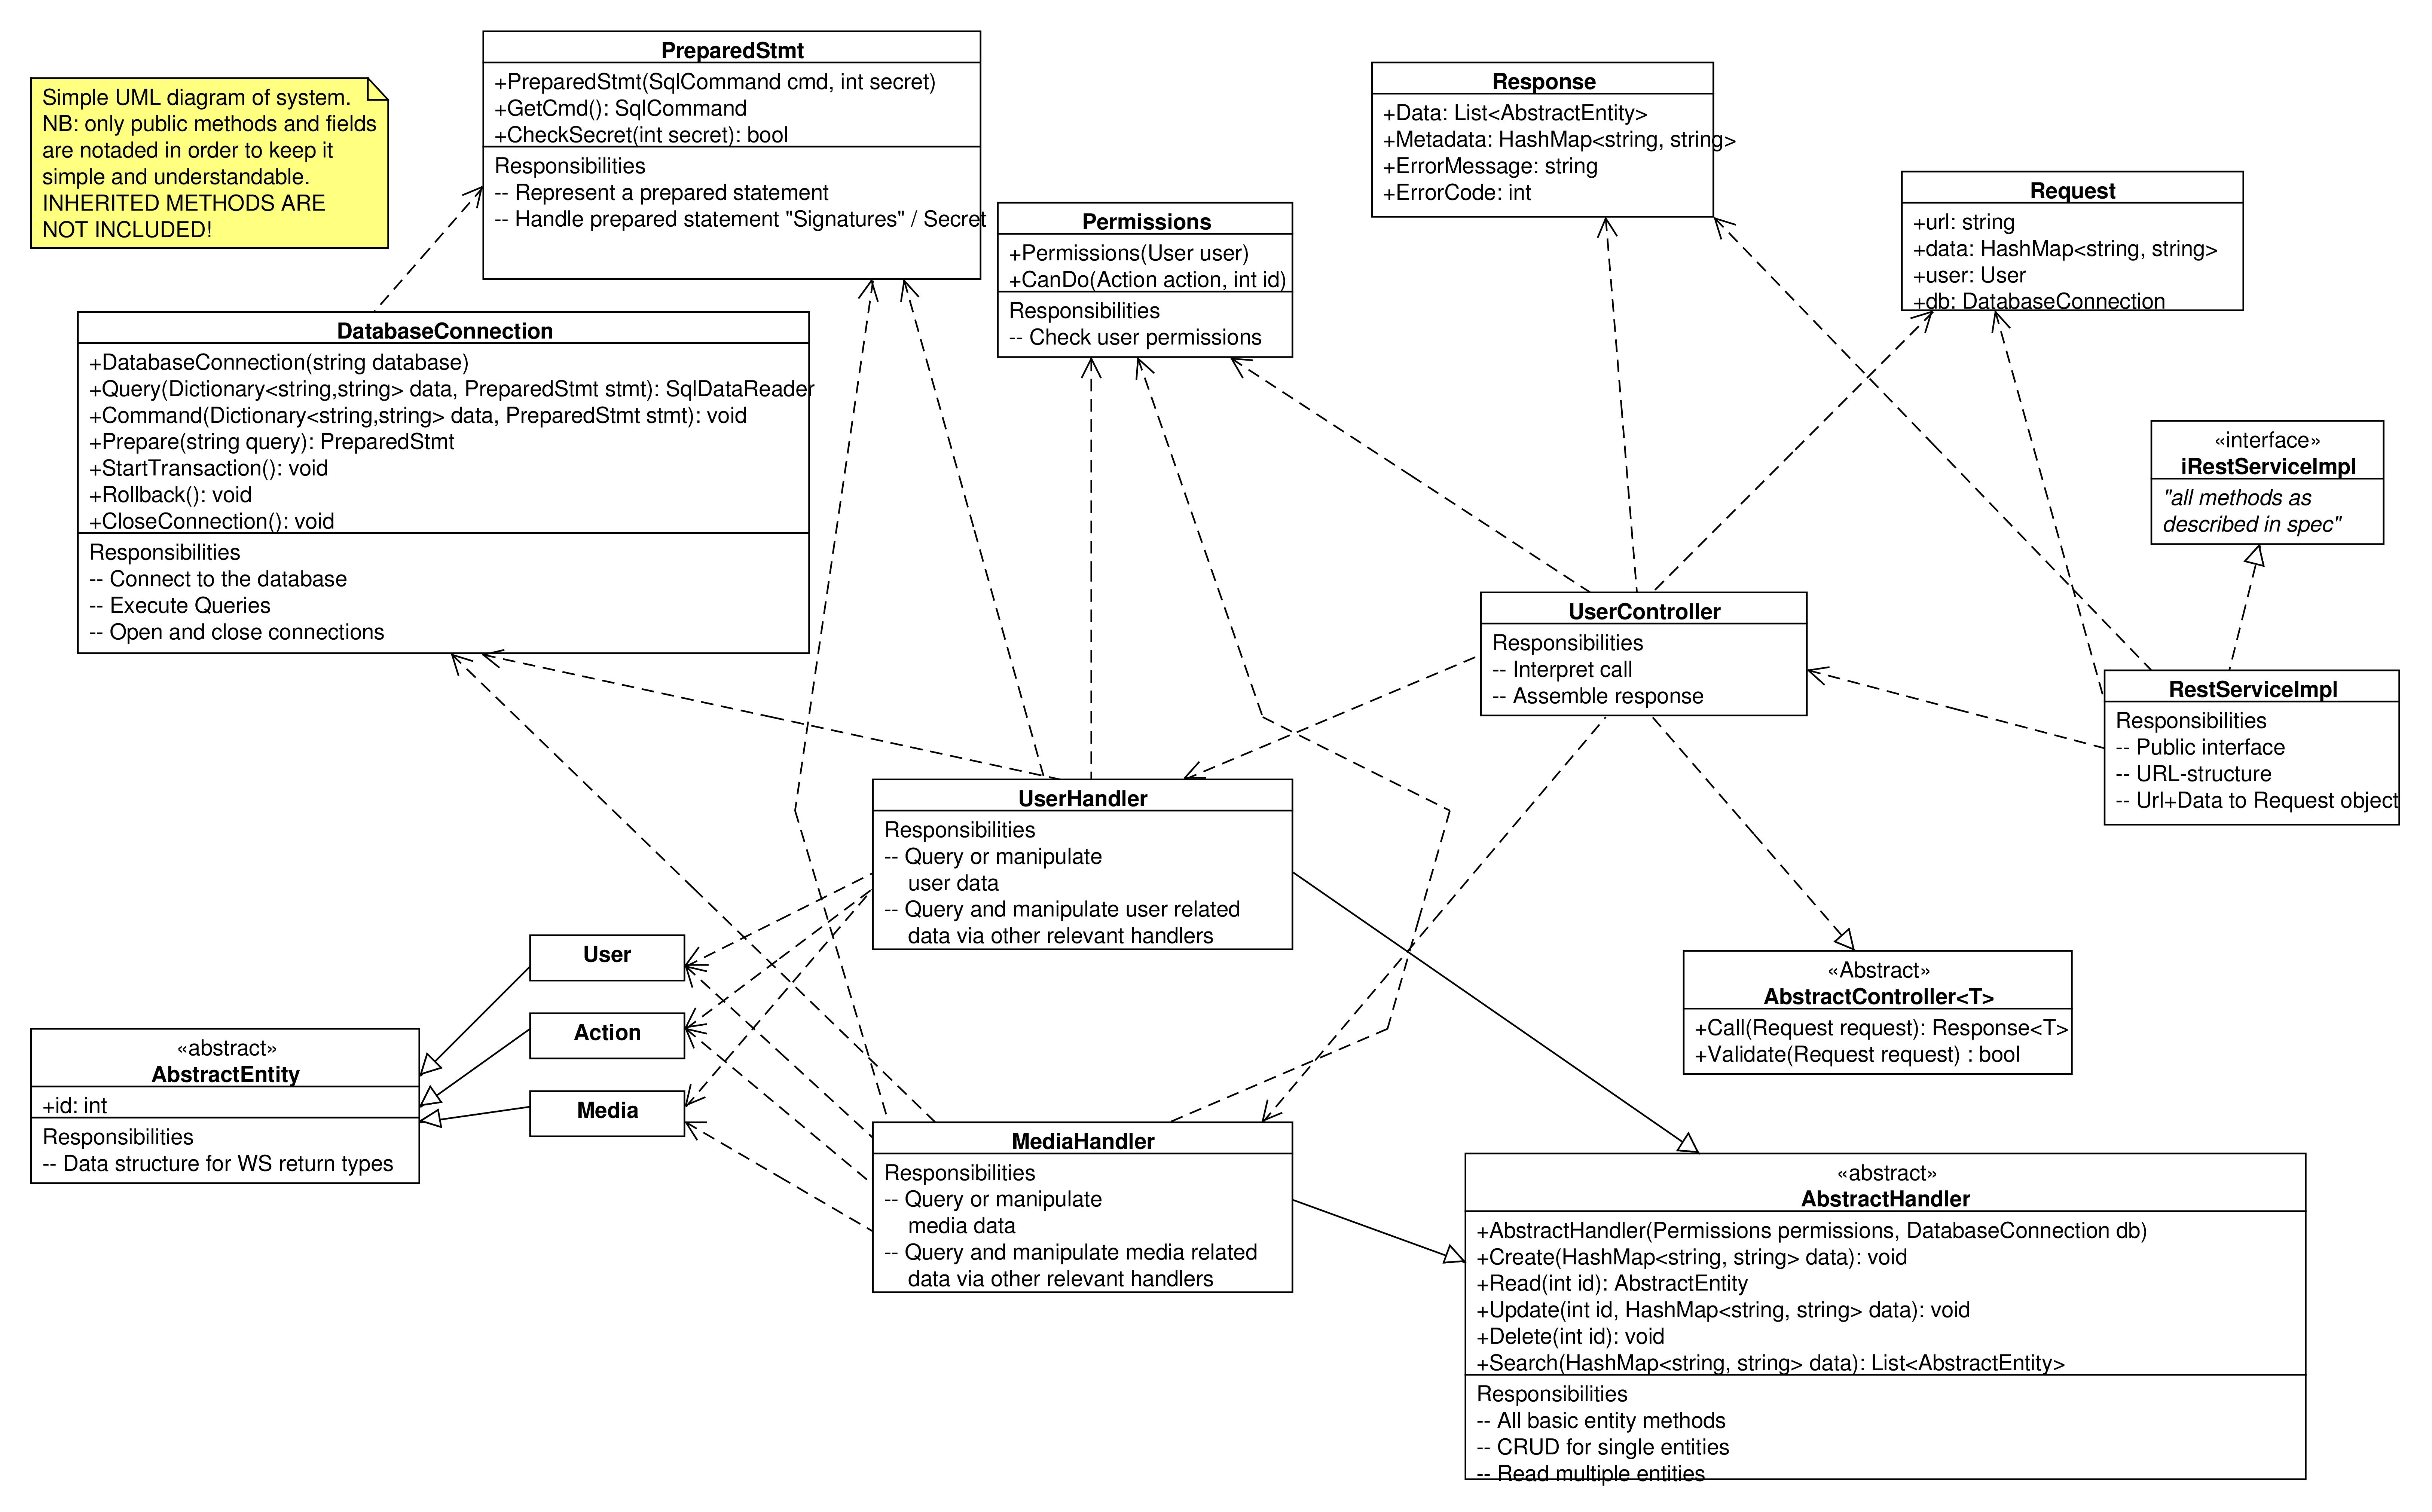
\includegraphics[width=1\textwidth, angle=270]{diagrams/class_diagram.jpg}
\end{figure}

\newpage

\section{Project Plan}

\begin{figure}[h!]
  \caption{Project plan for the ITU group}
  \centering
    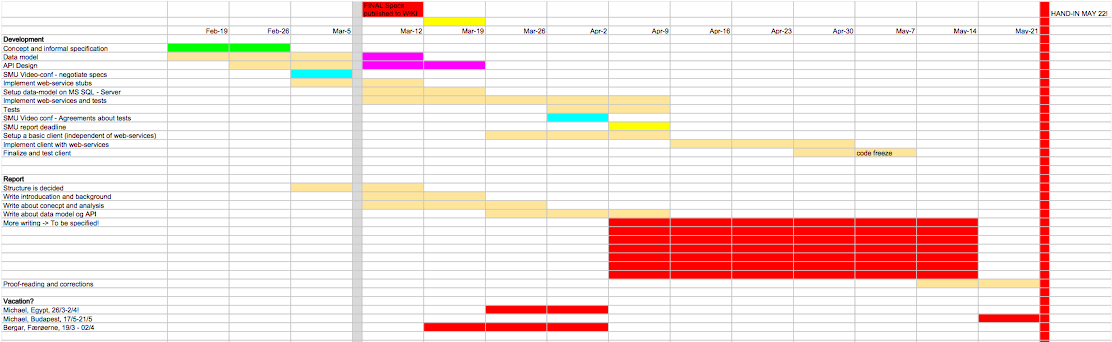
\includegraphics[width=1\textwidth, angle=270]{images/project_plan.png}
\end{figure}

\newpage

\section{Data Model}

\begin{figure}[h!]
  \caption{Complete data model for the system}
  \centering
    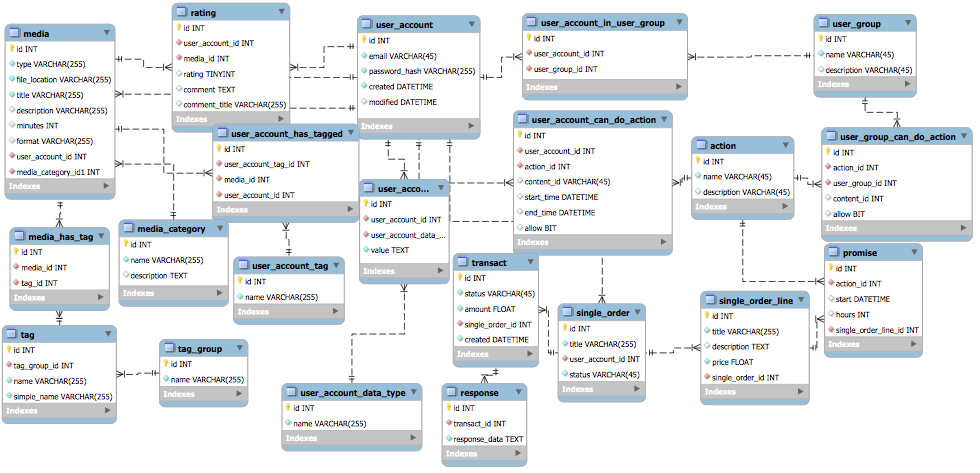
\includegraphics[width=1\textwidth, angle=270]{images/data_model.png}
\end{figure}

\end{document}
